\begin{pastexam}[label={px:df3-111-ds-05}]{地方三等資訊處理 111 年 第五題}
（申論；20 分）

下圖是一個加權圖 $G$=($V$, $E$)，其中 $V$ 是點集合而 $E$ 是邊集合。
\begin{center}
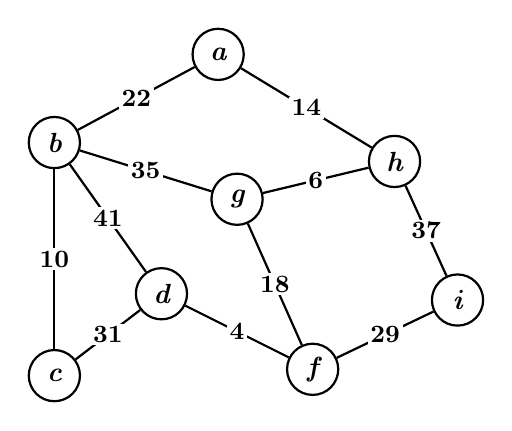
\begin{tikzpicture}[v/.style={circle,draw,thick,minimum size=6.5mm,inner sep=0pt,font=\bfseries\itshape},
  lab/.style={font=\small\bfseries,fill=white,inner sep=1pt}, thick, x=1.6cm, y=1.6cm]
\node[v] (a) at (1.3,2.9) {a};
\node[v] (b) at (0,2.2) {b};
\node[v] (g) at (1.45,1.75) {g};
\node[v] (h) at (2.7,2.05) {h};
\node[v] (d) at (0.85,1.0) {d};
\node[v] (i) at (3.2,0.95) {i};
\node[v] (c) at (0,0.35) {c};
\node[v] (f) at (2.05,0.4) {f};
\draw (a) -- node[lab] {22} (b);
\draw (a) -- node[lab] {14} (h);
\draw (b) -- node[lab] {35} (g);
\draw (g) -- node[lab] {6} (h);
\draw (b) -- node[lab] {41} (d);
\draw (h) -- node[lab] {37} (i);
\draw (b) -- node[lab] {10} (c);
\draw (g) -- node[lab] {18} (f);
\draw (d) -- node[lab] {4} (f);
\draw (c) -- node[lab] {31} (d);
\draw (f) -- node[lab] {29} (i);
\end{tikzpicture}
\end{center}
\begin{itemize}[leftmargin=2.2em, nosep]
\item[㈠] 請使用相鄰矩陣（Adjacency Matrix）表示法來表示加權圖 $G$。（5 分）
\item[㈡] 不考慮權重，從節點 $g$ 開始並按照字母順序對 $G$ 進行廣度優先尋訪（Breadth-First Search, BFS），請繪出尋訪完
後所產生的 BFS 樹（BFS Tree）。（5 分）
\item[㈢] 請利用 Prim's 演算法，從節點 $d$ 起始，找出一個最小擴張樹（Minimum Spanning tree），請以圖示方式一步步畫出
過程與結果，並說明 Prim's 演算法的時間複雜度。（10 分）
\end{itemize}
\end{pastexam}

\begin{pastsoln}
答案：㈡ BFS 樹：$g$ 的子節點 $b, f, h$；$b$ 的子節點 $a, c, d$；$f$ 的子節點 $i$。 ㈢ 依序加入 $(d,f)$ 4、$(f,g)$ 18、
$(g,h)$ 6、$(h,a)$ 14、$(a,b)$ 22、$(b,c)$ 10、$(f,i)$ 29，總權重 $103$；用二元堆積 $O(E \log V)$，用陣列 $O(V^{2})$。

（㈠㈡ 屬資結書第~21~章，㈢ 屬第~24~章。）

\textbf{㈠ 相鄰矩陣}（資結書第~21.2~節）：圖有 $8$ 個頂點 $a, b, c, d, f, g, h, i$（沒有 $e$），$11$ 條無向邊。 $M[u][v]$
是邊 $(u,v)$ 的權重，沒有邊記 $\infty$（對角線記 $0$ 或 $\infty$ 皆可，這裡記 $0$）；無向圖的矩陣對稱。
\begin{center}
\small
\begin{tabular}{c|cccccccc}
 & $a$ & $b$ & $c$ & $d$ & $f$ & $g$ & $h$ & $i$ \\ \hline
$a$ & 0 & 22 & $\infty$ & $\infty$ & $\infty$ & $\infty$ & 14 & $\infty$ \\
$b$ & 22 & 0 & 10 & 41 & $\infty$ & 35 & $\infty$ & $\infty$ \\
$c$ & $\infty$ & 10 & 0 & 31 & $\infty$ & $\infty$ & $\infty$ & $\infty$ \\
$d$ & $\infty$ & 41 & 31 & 0 & 4 & $\infty$ & $\infty$ & $\infty$ \\
$f$ & $\infty$ & $\infty$ & $\infty$ & 4 & 0 & 18 & $\infty$ & 29 \\
$g$ & $\infty$ & 35 & $\infty$ & $\infty$ & 18 & 0 & 6 & $\infty$ \\
$h$ & 14 & $\infty$ & $\infty$ & $\infty$ & $\infty$ & 6 & 0 & 37 \\
$i$ & $\infty$ & $\infty$ & $\infty$ & $\infty$ & 29 & $\infty$ & 37 & 0 \\
\end{tabular}
\end{center}

\textbf{㈡ BFS}（資結書第~21.3~節）：從 $g$ 開始，佇列先進先出；取出一個頂點後，依字母順序把還沒拜訪過的鄰居放進佇列，
並記下樹邊（父節點）。
\begin{center}
\begin{tabular}{lll}
\toprule
取出 & 新發現的鄰居（樹邊） & 佇列 \\
\midrule
（開始） & & $g$ \\
$g$ & $b, f, h$ & $b, f, h$ \\
$b$ & $a, c, d$（$g$ 已拜訪） & $f, h, a, c, d$ \\
$f$ & $i$（$d, g$ 已拜訪） & $h, a, c, d, i$ \\
$h, a, c, d, i$ & 鄰居都已拜訪 & 空 \\
\bottomrule
\end{tabular}
\end{center}
拜訪順序 $g, b, f, h, a, c, d, i$。 注意 $a$ 也和 $h$ 相鄰，但 $b$ 先被取出，所以 $a$ 的父節點是 $b$；$d$ 也和 $f$ 相鄰，
同理父節點是 $b$。 BFS 樹（每層是和 $g$ 的邊數距離）：
\begin{center}
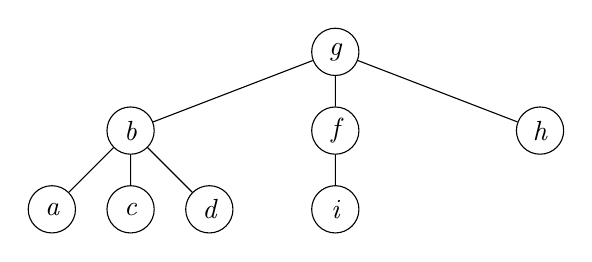
\begin{tikzpicture}[every node/.style={circle,draw,minimum size=6mm,inner sep=0pt,font=\itshape},
  level distance=10mm, level 1/.style={sibling distance=26mm}, level 2/.style={sibling distance=10mm}]
\node {g}
  child {node {b} child {node {a}} child {node {c}} child {node {d}}}
  child {node {f} child {node {i}}}
  child {node {h}};
\end{tikzpicture}
\end{center}

\textbf{㈢ Prim，從 $d$ 開始}（資結書第~24.3~節）：每一步在「一端在樹內、一端在樹外」的邊中選最輕的。
\begin{center}
\small
\begin{tabular}{clll}
\toprule
步 & 樹內頂點 & 跨出去的邊 & 選 \\
\midrule
1 & $d$ & $df$ 4、$dc$ 31、$db$ 41 & $(d,f)$ 4 \\
2 & $d, f$ & $fg$ 18、$fi$ 29、$dc$ 31、$db$ 41 & $(f,g)$ 18 \\
3 & $d, f, g$ & $gh$ 6、$fi$ 29、$dc$ 31、$gb$ 35、$db$ 41 & $(g,h)$ 6 \\
4 & $d, f, g, h$ & $ha$ 14、$fi$ 29、$dc$ 31、$gb$ 35、$hi$ 37、$db$ 41 & $(h,a)$ 14 \\
5 & $d, f, g, h, a$ & $ab$ 22、$fi$ 29、$dc$ 31、$gb$ 35、$hi$ 37、$db$ 41 & $(a,b)$ 22 \\
6 & $d, f, g, h, a, b$ & $bc$ 10、$fi$ 29、$dc$ 31、$hi$ 37 & $(b,c)$ 10 \\
7 & $d, f, g, h, a, b, c$ & $fi$ 29、$hi$ 37 & $(f,i)$ 29 \\
\bottomrule
\end{tabular}
\end{center}
每一步的樹（粗線是已選的邊，灰色是還沒選的邊）：
\begin{center}
\foreach \k in {1,...,7}{%
\begin{tikzpicture}[scale=0.8, v/.style={circle,draw,minimum size=4.5mm,inner sep=0pt,font=\scriptsize\itshape},
  lab/.style={font=\tiny,fill=white,inner sep=0.5pt}]
\node[v] (a) at (1.3,2.9) {a};
\node[v] (b) at (0,2.2) {b};
\node[v] (g) at (1.45,1.75) {g};
\node[v] (h) at (2.7,2.05) {h};
\node[v] (d) at (0.85,1.0) {d};
\node[v] (i) at (3.2,0.95) {i};
\node[v] (c) at (0,0.35) {c};
\node[v] (f) at (2.05,0.4) {f};
\foreach \u/\v in {a/b,a/h,b/g,g/h,b/d,h/i,b/c,g/f,d/f,c/d,f/i}{\draw[black!25] (\u) -- (\v);}
\foreach \u/\v [count=\j] in {d/f,f/g,g/h,h/a,a/b,b/c,f/i}{\ifnum\j>\k\else\draw[line width=1.6pt] (\u) -- (\v);\fi}
\node[font=\scriptsize] at (1.6,-0.35) {第 \k 步};
\end{tikzpicture}\hspace{1.5mm}}
\end{center}
最小擴張樹的邊：$(d,f)$、$(f,g)$、$(g,h)$、$(h,a)$、$(a,b)$、$(b,c)$、$(f,i)$，總權重
$4 + 18 + 6 + 14 + 22 + 10 + 29 = 103$。 權重都不同，最小擴張樹唯一（用 Kruskal 也得到同一棵，總權重 $103$）。

\textbf{時間複雜度。} Prim 要做 $V$ 次「找最輕的跨出去的邊」，並在每加入一個頂點後更新它的鄰居。
\begin{itemize}
\item 用陣列存每個樹外頂點到樹的最小距離：每次掃一遍找最小 $O(V)$，更新鄰居總共 $O(E)$，合計 $O(V^{2})$，適合
稠密圖或用相鄰矩陣時（資結書虛擬碼~24.5）。
\item 用二元堆積當優先佇列：$V$ 次取最小、最多 $E$ 次減少鍵值，每次 $O(\log V)$，合計 $O((V + E)\log V) = O(E \log V)$
（資結書虛擬碼~24.3）；用 Fibonacci 堆積可以降到 $O(E + V \log V)$。
\end{itemize}
本題用相鄰矩陣表示，掃一列就是 $O(V)$，所以用陣列版是 $O(V^{2})$。
\end{pastsoln}
